
\section{CUDA synchronization mechanisms}

As we've discussed in the section on architecture, when writing kernels, we need always to think about the GPU's hardware, scheduling, etc...
By now, with the basic examples we've considered only \textit{basic} operations. Indeed, the only API function we've used in the kernel is the \verb|__syncthreads()|. 
This is a simple syncing mechanism, that ensures that all the threads \textbf{within the block} are 
done before this barrier. This is block-level synchronization barrier.

\subsection{Cooperative Groups}

\begin{listing}
\begin{minted}[frame=single, linenos=true]{cuda}
__device__ int reduce_sum(
    cooperative_groups::thread_group gr, \
                        int *temp, int val){
    int lane = g.thread_rank();

    for (int i = g.size() / 2; i > 0; i /= 2){ 
//map each element in the first "semi" block 
//to it's corresponding element in the second one
        temp[lane] = val;
        g.sync(); // wait for all threads to store
        if(lane<i) val += temp[lane + i];
        g.sync(); // wait for all threads in to load
    }
    return val; //only thread 0 will return full sum
}
\end{minted}
\label{coop_group}
    \caption{This method, is \sout{almost} the same as the first, optimized version of the reduce 
    algorithm, using the shared memory \autoref{}. Therefore, one must note that this reduce\_sum() method 
    must be called for the array temp*, located in the shared memory.}
\end{listing}


Cooperative groups is a relatively new feature to the CUDA API.
As the name suggests it, this feature enables us to group threads, with the 
ability to perform common, collective operations (or simply collectives). We can also 
perform synchronization between the threads, belonging to the same cooperative groups. 
With these API features, one can simplify the code, thus avoiding common mistakes and make it more readable.
For example, in the code snippet 
\autoref{coop_group}, we perform the exact same algorithm as in \autoref{shatred_mem_optim1},
by using some utility of the CUDA API. In this case, the \verb|cooperative_groups::thread_group|
class (do not pay attention to how we created this object and/or how it is declared).
The \verb|thread_rank()| function gets the ID/rank of the thread within the thread group \verb|g| (the same way as \verb|threadId.x| within a block). 
Then we're calling the \verb|sync()| function, which ensures that all the threads within the thread group 
will be done setting the \verb|val|, and the second to ensure that all threads are done reducing. It is important to understand, that all the threads will return the val. 
However, only the thread 0 will accumulate all the \verb|val|'s.\cite{blog_2020}

\subsection*{Thread blocks}
We've already seen the notion of a thread block many times. This notion was always quite \textit{abstract}. Indeed, while launching the kernel, we've 
always kept the notion of thread blocks in our mind, but never actually accessed it. However, in newly introduced features, we can "access" the 
thread block explicitly. Remember the legacy \verb|__syncthreads()| function. 
Well, syncing the \verb|this_thread_block()| does the same thing as the \verb|__syncthreads()|. Thus, there are several ways/semantics to synchronize the threads. 
The following function calls are synonyms.


\begin{listing}
\begin{minted}[frame=single]{cuda}
    auto tb = this_thread_block(); // gets the thread block in kernel
    tb.sync() // same method as in cooperative_groups
    cooperative_groups::synchronize(tb);
    this_thread_block().synchronize();
    cooperative_groups::synchronize(this_thread_block());
\end{minted}
\end{listing}

One can also mention other synonyms \verb|dim3 threadIdx| $\equiv$ \verb|dim3 thread_index()| and \verb|dim3 blockIdx| $\equiv$ \verb|dim3 group_index()|. Thus one can easily replace 
these built-in keywords with these new methods, without any noticeable performance issues.

\subsection*{Partitioning}
For these cooperative groups, a partitioning feature is also avaliable. For instance, if 
we've created a thread thread block, by invoking \verb|auto tb = this_thread_block()|,
one can divide it into more small parts, for instance, into groups of 16 threads. 
This is done using the \verb|cooperative_groups::partition()|, method, which takes the 
subject itself (the one to be partitioned into groups) and the number of threads per group.
For instance, \verb|cooperative_groups::partition(tb, 16)| divides the thread block into 
groups of 16 threads (so if e.g. a block has a max of 64 threads, this function will create)
4 groups of 16 threads in each. 

The object returned is a \verb|thread_group|. By accessing this object, it is possible to get 
the thread's rank, \textbf{within the obtained thread\_group} (for instance, if we divide 
the thread block into groups of 16 threads and, by passing this object to a device function,
print the \verb|thread_rank()|, method, we will see numbers varying from 0 to 15). 

The utility of these features overall is that it is less easier to make errors. Indeed, 
the NVidia documentation states that the usage of these features significantly reduces the 
risk of deadlocks. The concept of deadlocks is probably well known to the reader. This is 
a typical situation, when we don't want different threads to access a critical section, and 
ask them to be synchronized before accessing them. Consider the two pieces of code:

\begin{listing}[!ht]
\begin{minted}[frame=single, framesep=1mm]{cuda}
__device__ int sum(int *x, int n) 
{   ...
    __syncthreads();
    ...
}
__global__ void parallel_kernel(float *x, int n)
{
    if (threadIdx.x < blockDim.x / 2){
        sum(x, count);  // Half of the threads enter and 
                        //the other half-not
    }                   
}
\end{minted}
\caption*{}
\label{deadlock}

\begin{minted}[frame=single, framesep=1mm]{cuda}
__device__ int sum(thread_block block, int *x, int n) 
{   ...
    block.sync();
    ...
}
__global__ void parallel_kernel(float *x, int n)
{
    sum(this_thread_block(), x, count); //OK
}
\end{minted}
    \caption{Synchronizing using the legacy mechanism \textit{vs} using the cooperative groups. \cite{blog_2020}}
\label{nodeadlock}
\end{listing}

\newpage
In a nutshell, we clearly see a deadlock in the first piece of code, as 
there are only threads with ID's less than the half of the block dimension, which will 
enter the if condition. Those threads will perform their piece of code independently, 
and then will wait for all the other threads in the block to be completed and 
synchronized. This is a big issue, as there are threads, which will never start the \verb|sum()|
kernel and will just sit up there, waiting for those, who have. So the two chuncks of threads
will just wait for each other. 

This is why one may find an application for the previously discussed primitives. 
In the second piece of code, one call the method \verb|sum()| with a thread block. However, 
we could have divided into groups, using either CUDA functionality discussed above, 
\textbf{and only synchronize that block}, which, we are sure, will by run by all threads in 
the block. 

\subsection*{Warp synchronizations}
%https://blog.csdn.net/jqw11/article/details/103071556
While programming with CUDA, one never gets tired to tired to think about warps, and 
how to optimize their execution. I do agree that it is not an easy task, to think of it, 
while doing even some basic operations. The new NVidia architectures and new versions of the
CUDA API, provide a simple way to navigate through these concepts.

We have discussed a lot the advantages of the shared memory (e.g. for the speed and efficiency
of the reduce algorithm). However, the new utilities give us a more faster, or even a more
local way to perform some operations. Remember, shared memory is block-local memory. 
Remember also that every thread has some kind of register to store small intermediate 
values while performing a kernel, for example, when
we used to store the local thread ID. 
The so called \textit{warp level synchronization primitives}
allow us to access a certain thread's local register from an another thread,
\underline{as long as they are in the same warp}, without 
the usage of the shared memory. Again, there are many things to keep in mind, 
but if such a function is called, it is doing everything \textit{atomically}, 
in the sense that it is a primitive operation, performed locally on the threads in the 
warp. We therefore introduce here the notion of the 
\textbf{lane} (in fact, we used it briefly above). A lane is the thread id within the warp.
%https://on-demand.gputechconf.com/gtc/2013/presentations/S3174-Kepler-Shuffle-Tips-Tricks.pdf


\paragraph{A little disclaimer: }There are various Warp-level primitive functions. We will note that many function's
name are similar, and only differ by the postfix \verb|_sync()|. For instance, 
\verb|__shfl_xor()| and \verb|__shfl_xor_sync()|. Indeed, the ones with the \verb|_sync()|
postfix is a improvement of the former. It is recommended to use the newer version instead.
I will not go into great details between these differences. 
I will just mention that there are differences in parameters
\footnote{Frankly speaking, the author hasn't seen this additional parameter 
being used in a very extensive way. This \textit{extra} parameter is often replaced with 
some kind of hardcoded value}(see further examples).


The \verb|__activemask()| primitive/function is actually not a synchronization 
mechanism, but more of a filtering mechanisms. This function returns the \textit{indices}
of the active threads in the warp, where it was referenced from\footnote{One can think 
of the mask as the python's numpy feature, while doing a filter : {\fontfamily{pcr}\selectfont arr[:]<1.0}, which 
will return an array of booleans, which will be used to access later the elements of interest}. 
So the result returned from the \verb|__activemask()| is used to call other synchronization functions, 
to \textit{give them the corresponding threads, that are active in the warp}.
So, for example, one could call the  \verb|__syncwarp(MASK)|, thus asking 
to sync all the threads meeting the \verb|__activemask()| condition. 
One can go to the NVidia's developer's guide \cite{center} and find the following:

\begin{quote}
    \textsl{
Returns a 32-bit integer mask of all currently active threads in the calling warp. 
The Nth bit is set if the Nth lane in the warp is active when \_\_activemask() is called. 
Inactive threads are represented by 0 bits in the returned mask.
    }
\end{quote}

So let's have a quick look and example at what did NVidia provide us with 
\footnote{There are many such primitives available. As usual, the best way to get information about such 
CUDA functionality, is to look it up in the NVidia's developer's guide \cite{center}.}

\begin{itemize}
    \item \verb|__shfl_sync()| or in previous CUDA versions \verb|__shfl()| is a tool, to "broadcast", or "spread"
        a certain value from a certain thread (identified with its lane) to all others in the warp. For example, 
        in a certain warp, all the threads have a variable \verb|int b = //some random int|, unique for all 
        the threads. And I want all these thread's variable \verb|b|, to be the same as the one in the thread 
        4 (its lane number or ID within the warp). The best way to do that is to use the provided function:
        \verb|__shfl_sync(0xffffffff, b, 4)| (or \verb|__shfl(b,4)|). The second parameter is the variable to be 
        broadcasted and the third one is the lane number to take the value from (because, of course, all the 
        threads have this local variable \verb|b|, which is different for all of them). So we're replacing all the 
        b's with THE b of the thread 4. The first parameter is actually the mask/filter, that tells the 
        processor (or core I should say) which threads will be involved in this operation. This can be used 
        by passing the result of e.g. \verb|__activemask()| function (there are multiple \textit{filtering} functions)
        or by passing it the \textit{default} value in hex notation, which corresponds to the maximum number 
        that can be displayed in binary notation (all the 32 bits are 1, thus we're saying that all the threads are active).

    \item \verb|__shfl_up_sync()| or in previous CUDA versions \verb|__shfl_up()| is a function to 
        shift the values of the warp by an offset. For instance, let's say that in the warp, I want 
        the 4'rd thread to have the value from 0'th thread, the 5'th thread the value of the 1'st, the 6'th 
        thread the value from the 2'nd thread, etc ... Then we would want to use the \verb|__shfl_up_sync()| 
        function, with the same parameters as in the \verb|__shfl_sync()| function described above.
    \item \verb|__shfl_down_sync()| Is the same idea as the \verb|__shfl_up_sync()|. The difference is that 
        we would use it if we wanted e.g. the thread 29 to have the value 31. (see figure for better understanding).
\end{itemize}

These primitives come in various shapes and forms. It would take quite a time
to discuss them all here. The idea for them all, however, follows quite well the 
patterns, we've discussed just above. It is important to understand that these operations
are sort of atomic, because, as we've seen, these are warp-local primitives, which is the most 
fundamental part of the execution scheduling model.


\subsubsection*{Atomics}
When learning multithreaded programming, one of the first notions, that one must understand
is the notion of atomics or atomic operations \footnote{Intuitively, 
this comes from the word \textit{atom}. This is a greek word, meaning something 
like \textit{uncuttable}, \textit{undivisible}. In fact, this is almost exactly, what an atomic operation corresponds to 
\cite{atomics} .}
. To make it short, these operations are operations, which, we are sure, will be performed \textit{in the smallest possible
period} and nothing will be able to affect the execution of these operations.
For example, in C++, there is a \verb|std::atomic<bool>| template specialization. 


In the CUDA API, multiple atomic operations are provided. Arithmetic atomic operations, 
such as \verb|atomicAdd()|, \verb|atomicSub()|, \verb|atomicMin()|, ... 
,bitwise functions, such as \verb|atomicAnd()|, \verb|atomicXor()|, ...
(for more: \cite{center}).
All these operations have the same (or almost same) signatures: 
\verb|int <or any primitive type> <function_name>(int* old_adress, int value)|
So these functions take the old adress as the first parameter (for example, the address of the value, we want to add to) and 
the value as the second. The function thus performs an arithmetic or logical operation atomically, 
and stores the result in the old adress. It also returns the value.


The atomic operations are however very expensive, as the scheduler must perform sequentialize the memory access. 
It is thus very advisable to use these operations, only when needed.
For example, let's say we've performed some kind of reduction on multiple blocks locally. 
We know that if we've used some shared of memory on this reduction, one must in addition add the block results, to 
get the full answer of our reduction. One way to do that is to force an atomic operation in all blocks, so they store it 
in the first address of the global memory, that we will later \textit{consume} from the CPU. 
So if one  suppose that we've accumulated the thread-local reduce into \verb|sum| and the pointer to the 
initial data \verb|g_out|, we would do something like

\begin{minted}[frame=single]{cuda}
    if(this_thread_block().thread_rank()==0){
        atomicAdd(&g_out[0], sum);
    }
\end{minted}


\section{Streams}
\label{sec:streams}
\subsection{Concept of streams}
CUDA streams is an another fundamental concept that we've used previously in an implicit manner.
Indeed, let me provide an another example using C++: when a "Hello World" programm is written in C++, 
no one cares about the thread usage. We do not create a "main" thead, when printing a character to 
the standart output. In the context of the CUDA API, \textbf{any} programm is by definition multithreaded. 
Therefore the analogy between the \textit{usual} C/C++/Python/... and a GPU programm does not make sense.
The stream concept is more of a thread \textbf{over the GPU threads}. 
By now, all the programs we've considered were launched in one single CUDA stream. So one can launch a 
programm (e.g. a simple vector addition) in one stream, which will be performed in parallel. However one can 
add a second vector addition programm, which will be done in parallel, with the first vector addition.



A CUDA stream is thus a way to make two (or more) kernels run in parallel. (Remember that the kernels 
themselves are already run in parallel following the CUDA architecture). By now, we've used one implicit stream - the default stream.

\subsection{Basic usage of streams}
Let's try to explicitly create a stream and look at its initialization syntax:

\begin{listing}[ht!]
\begin{minted}[frame=single]{cuda}
    cudaStream_t stream;
    cudaStreamCreate(&stream);
    foo_kernel<<< grid_size, block_size, 0, stream>>>();
    cudaStreamDestroy(stream);
\end{minted}
\end{listing}

Therefore to create the CUDA stream, one must first initialize the stream, then create the stream, i.e. 
allocate the memory via the \verb|cudaStreamCreate()| method by passing the pointer of the stream. 
In order to call the kernel and make it run in a particular stream, one pass it as the last parameter in the angle brackets.
If nothing is passed in the in the angle brackets for the stream, the default stream is used.

The simplest usage example of cuda streams is when one would want to concecutively call a certain kernel multiple times 
(for example N times). 
the way to do it using the default stream is to simply loop N times and call the kernel at every iteration.
The way to do it using streams, is to create an array of streams and call the kernel by assigning it to different streams.
The kernels will then be run in parallel without waiting the previous kernel return. The execition of the kernels 
So these functions take the old adress as the first parameter (for example, the address of the value, we want to add to) and 
the value as the second. The function thus performs an arithmetic or logical operation atomically, 
and stores the result in the old adress. It also returns the value.


The atomic operations are however very expensive, as the scheduler must perform sequentialize the memory access. 
It is thus very advisable to use these operations, only when needed.
For example, let's say we've performed some kind of reduction on multiple blocks locally. 
We know that if we've used some shared of memory on this reduction, one must in addition add the block results, to 
get the full answer of our reduction. One way to do that is to force an atomic operation in all blocks, so they store it 
in the first address of the global memory, that we will later \textit{consume} from the CPU. 
So if one  suppose that we've accumulated the thread-local reduce into \verb|sum| and the pointer to the 
initial data \verb|g_out|, we would do something like

\begin{minted}[frame=single]{cuda}
    if(this_thread_block().thread_rank()==0){
        atomicAdd(&g_out[0], sum);
    }
\end{minted}

\subsubsection{Asynchronous streams}

We've already mentioned the asynchronous memory transfer mechanism, when discussing the memory models (see \ref{subsub:async_mem}).
Let's get back to the same example, and illustrate in more detail on what was happening in the codes.
\begin{listing}
  \begin{minted}[frame=single, framesep=1mm, linenos=true]{cuda}
  for (int i = 0; i < nStreams; ++i){
    int offset = i * streamSize; //offset for memory copy 
    cudaMemcpyAsync(&d_a[offset], &a[offset], streamBytes,\
      cudaMemcpyHostToDevice, stream[i]);
    kernel<<<streamSize/blockSize, blockSize, 0,\
      stream[i]>>>(d_a, offset);
    cudaMemcpyAsync(&a[offset], &d_a[offset], streamBytes,\
      cudaMemcpyDeviceToHost, stream[i]);
  }
  \end{minted}
  \label{fig:async_mem_streams}
\end{listing}
\end{itemize}

Without the streams and the asynchronous memory copy, all the operations invoked in the loop would have been sequential. Suppose 
that one of requirements is not fulfilled. That is, suppose one replaces the \verb|cudaMemcpyAsync()| with something else, and/or remove the stream functionality.
Then the iteration of \verb|i=1| will wait for the \verb|i=0| iteration and so on (see \ref{fig:async_mem_streams}).

\begin{figure}
  \centering 
  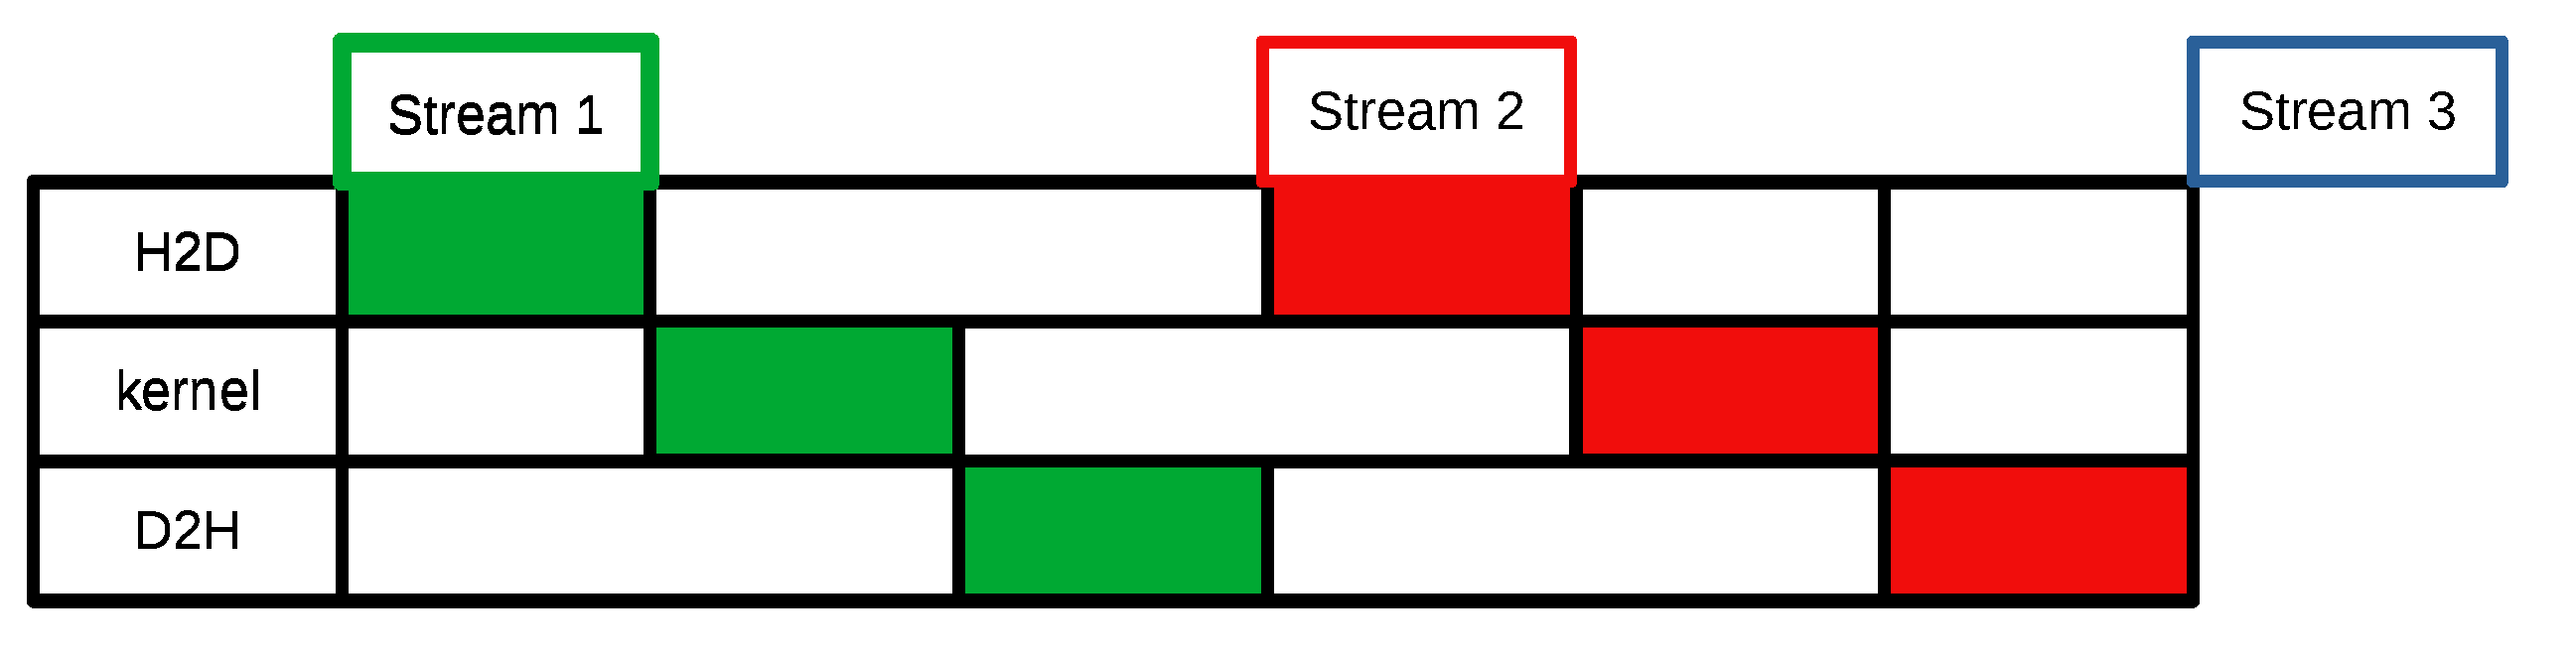
\includegraphics[scale=0.15]{pngs/asyncmem-page1.png}
  \caption{Scenario of the execution pipeline, if no streams and asynchronous memory are involved.}
\end{figure}

One may see that the sequential version does not fully use the potential of the GPU. That is, some of the memory 
transfer mechanisms are waiting for others to finish. To solve this problem, one use the asynchronous memory version (\ref{fig:async_mem_streams}).
In this case, the execution pipeline would look like that:

\begin{figure}
  \centering 
  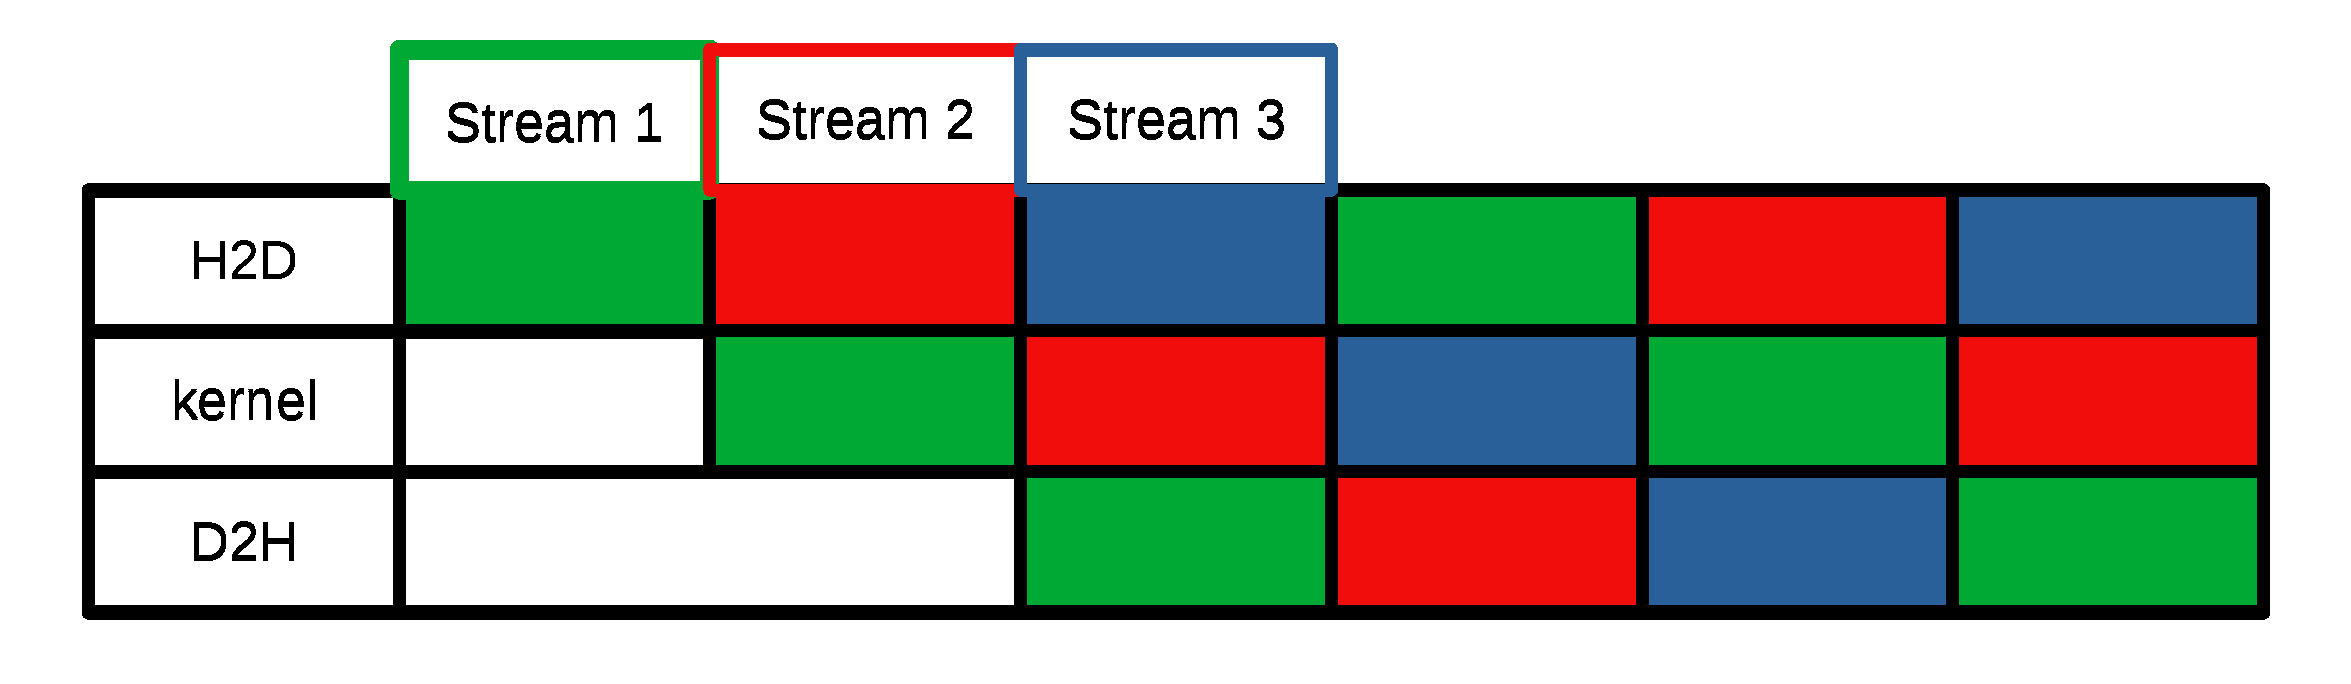
\includegraphics[scale=0.15]{pngs/asyncmem-page2.png}
  \caption{Scenario of the execution pipeline, which is fully asynchronous and fully uses the memory transfer mechanism's resources.}
  \label{fig:fully_async_mem}
\end{figure}

Note that this \ref{fig:fully_async_mem} pipeline is not always true. That is, based on different architectures, 
different results can be expected. For example, some of the versions have only a single memory copy and kernel engines. 
This implies that the async functionality does not make sense for these versions (note that these versions are not very common anymore).







